\PostFigureHeadingSpace
\section{System Validation Results}

This section evaluates whether the reconstructed system preserves its operating contracts in the bounded reference slice. The validation checks whether source grounding, routing, trace completeness, output hygiene, interface connectivity, and latency remain under engineering control.

\subsection{Validation Protocol}

Each fixed validation scenario is a versioned test case: one investor-facing question, an entity scope, expected claims, required answer signals, trace requirements, prohibited patterns, and a latency budget. It passes only when all required evidence and trace fields resolve and no configured blocker fires.
The scenario questions are product-facing briefing prompts, not expert-approved investment recommendations. Some prompts use terms such as investment point because the motivating demonstration needed questions that were recognizable to business users; in this paper, those prompts test routing, evidence selection, answer structure, and trace preservation.

The role of each contract area is defined in \Cref{tab:enterprise-validation-frame}. Prompt, model, and output evaluation tools measure important application behavior; the reconstructed architecture adds a product-control layer for source authority, entity scope, trace retention, and user-facing constraints.

\begin{table}[H]
    \centering
    \caption{Contract frame for system-level assessment.}
    \label{tab:enterprise-validation-frame}
    \footnotesize
    \setlength{\tabcolsep}{4pt}
    \renewcommand{\arraystretch}{1.20}
    \begin{tabular}{@{}C{0.20\linewidth}
                    L{0.39\linewidth}
                    L{0.31\linewidth}@{}}
        \toprule
        \multicolumn{1}{C{0.20\linewidth}}{Contract area} & \multicolumn{1}{C{0.39\linewidth}}{Requirement} & \multicolumn{1}{C{0.31\linewidth}}{Evidence reported} \\
        \midrule
        Source grounding & Runtime answers must remain tied to registered sources and promoted claims. & Claim-reference and trace-field outcomes in \Cref{tab:validation-results}. \\
        Entity and answer scope & Fixed scenarios must preserve entity scope, required answer signals, and prohibited-language constraints. & Scenario outcomes in \Cref{tab:validation-results} and the fault-injection sensitivity check in \Cref{sec:fault-injection-sensitivity}. \\
        Output hygiene & User-facing answers must stay separated from internal traces while preserving source links and answer structure. & Answer and gate outcomes in \Cref{tab:validation-results}. \\
        Runtime interfaces & Live interfaces and orchestration should connect to external sources while preserving the answer contract. & Live-interface outcomes in \Cref{sec:runtime-interfaces}; latency outcomes in \Cref{tab:latency-results}. \\
        \bottomrule
    \end{tabular}
\end{table}

The fixed validation slice contains 30 investor-facing scenarios: five selected-company questions and one cross-company comparison for each of the five corporate-group slices. Appendix~\ref{app:scenario-inventory} gives the scenario inventory, question-design rules, and representative question examples.

\subsection{Scenario Contract Outcomes}

Fixed validation scenarios test whether the system preserves its source, routing, trace, and answer-structure contracts. They are narrower than full RAG evaluation \citep{es2023ragas,saadfalcon2024ares,liang2023helm}; their role is to fix a reproducible baseline for contract preservation. The aggregate outcomes for the six fixed questions per corporate group are reported in \Cref{tab:validation-results}. Each corporate group uses the same question design: five selected-company questions plus one cross-company comparison. Each result cell reports passing configured checks over required checks.

\vspace{-0.25\baselineskip}
\begin{table}[!htbp]
    \centering
    \caption{Fixed validation-scenario contract results.}
    \label{tab:validation-results}
    \footnotesize
    \setlength{\tabcolsep}{6pt}
    \renewcommand{\arraystretch}{1.12}
    \begin{tabular*}{0.98\linewidth}{@{\extracolsep{\fill}}C{0.20\linewidth}cccccc@{}}
        \toprule
        \multicolumn{1}{C{0.20\linewidth}}{Corporate group} & Scenarios & Claim refs & Trace & Answer & Hygiene & Failed \\
        \midrule
        Samsung & 6/6 & 25/25 & 6/6 & 6/6 & 12/12 & 0 \\
        SK & 6/6 & 30/30 & 6/6 & 6/6 & 12/12 & 0 \\
        Hyundai Motor & 6/6 & 20/20 & 6/6 & 6/6 & 12/12 & 0 \\
        LG & 6/6 & 20/20 & 6/6 & 6/6 & 12/12 & 0 \\
        Hanwha & 6/6 & 14/14 & 6/6 & 6/6 & 12/12 & 0 \\
        \midrule
        Total & 30/30 & 109/109 & 30/30 & 30/30 & 60/60 & 0 \\
        \bottomrule
    \end{tabular*}
    \vspace{0.10em}
    \begin{minipage}{0.94\linewidth}
        \footnotesize
        Cells report passed checks over required checks. \textit{Claim refs} counts expected source-backed claim references. \textit{Trace}, \textit{Answer}, and \textit{Hygiene} check the audit envelope, visible answer contract, and leakage/link controls.
    \end{minipage}
\end{table}
\vspace{-0.35\baselineskip}

Within the bounded reference slice, all configured source, trace, answer, and output-hygiene contracts passed. The 109/109 source-claim result means that every expected evidence reference in the scenario files resolved to a promoted claim. The 30/30 trace-contract result means that every answer preserved the required audit envelope. The 30/30 answer-contract result means that every visible answer contained the required answer signals and avoided prohibited patterns. The 60/60 output-hygiene result means that internal-trace leakage was blocked and user-visible source links were preserved across the 30 scenarios. The 0 failed runs result means that no scenario was stopped by a configured blocker. The corresponding evaluator artifacts are stored in the repository's \path{evals/results/} directory.

The user-facing answer view associated with these checks is shown in \Cref{fig:ui-mobile-answer}. The visible answer summarizes financial metrics, risks, and monitoring points while keeping comparative items bounded by the answer contract. The source-link and follow-up region is shown in \Cref{fig:representative-answer-output}.

\begin{figure}[H]
    \centering
    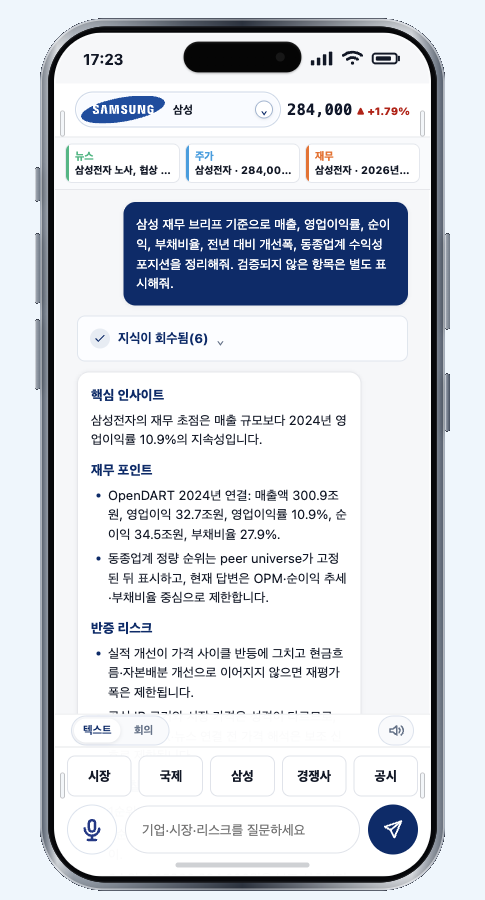
\includegraphics[width=0.49\linewidth]{figures/ui_mobile_answer_ko.png}
    \caption{Mobile answer view for a fixed finance-brief scenario. The retrieved-knowledge marker denotes a loaded evidence package; the answer uses insight-first sections with internal trace artifacts kept in the audit layer.}
    \label{fig:ui-mobile-answer}
\end{figure}

\subsection{Fault-Injection Sensitivity}
\label{sec:fault-injection-sensitivity}

Here, fault injection refers to mutating one contract property at a time to test validator sensitivity. Starting from one valid scenario, seven mutated copies were evaluated with the same contract checks. The validator detected all seven induced violations and missed none. The concrete mutation protocol is shown in \Cref{tab:fault-injection-protocol}, and the full artifact is stored under the repository's \path{evals/results/} directory. When key contract properties are deliberately broken, the corresponding validators fail the run.

\subsection{Runtime Interfaces and Orchestration}
\label{sec:runtime-interfaces}

After fixed-scenario validation, the implementation was exercised with live filing, market, and news interfaces. Runtime interface checks passed 5/5 live API corporate-group connectivity checks and 15/15 live answer-hygiene checks, with inspection packets generated for all 15 runtime samples. These checks verify interface wiring and artifact hygiene.

Latency was measured on the 14 scenarios that had paired baseline and optimized measurements in the May 3 latency dashboard. The optimized run used parallel source collection and process-level caching for repeated source reads. As shown in \Cref{tab:latency-results}, mean latency decreased from 2008.57ms to 171.14ms, and the number of runs under the fixed 1500ms engineering budget increased from 2/14 to 13/14. The budget is used as an internal runtime threshold for these fixed scenarios. The measurements use the deterministic composer; live-LLM provider latency is outside this comparison. These results show that the same answer contract can be preserved while the runtime moves from static artifacts toward live source interfaces and optimized orchestration.

\begin{table}[!htbp]
    \centering
    \caption{Fixed-scenario latency before and after runtime optimization.}
    \label{tab:latency-results}
    \footnotesize
    \renewcommand{\arraystretch}{1.12}
    \begin{tabular*}{0.96\linewidth}{@{\extracolsep{\fill}}C{0.31\linewidth}C{0.25\linewidth}C{0.25\linewidth}@{}}
        \toprule
        \multicolumn{1}{C{0.31\linewidth}}{Measure} & \multicolumn{1}{C{0.25\linewidth}}{Baseline run} & \multicolumn{1}{C{0.25\linewidth}}{Optimized run} \\
        \midrule
        Scenario count & 14 & 14 \\
        Average latency & 2008.57ms & 171.14ms \\
        Median latency & 2156ms & 86ms \\
        p90 latency & 2467ms & 143ms \\
        Runs under 1500ms budget & 2/14 & 13/14 \\
        \bottomrule
    \end{tabular*}
\end{table}
